% Set document class to article and font size to 11pt.
\documentclass[11pt]{article}

%================================================================================%
%                                  PACKAGES                                      %
%================================================================================%
%--------------------------------%
%     MATH AND FONT PACKAGES     %
%--------------------------------%
% Math fonts
\usepackage{amsfonts}
% Math symbols and environments
\usepackage{amsmath}
% More math symbols
\usepackage{amssymb}
% More math tools (like the mini matrix)
\usepackage{mathtools}
% Dirac bra-ket notation
\usepackage{braket}
% Bold face
%\usepackage{bbold}
% A better bold face
\usepackage{bm}
% \mathds for double stroke font for fancy unitary 1
\usepackage{dsfont}

%-------------------------%
%     FIGURE PACKAGES     %
%-------------------------%
% Create figures with captions
\usepackage{graphicx}
% Figure labels/titles are bold
\usepackage[labelfont=bf]{caption}
% Subfigure environments
\usepackage{subcaption}

%-----------------------------%
%     FORMATTING PACKAGES     %
%-----------------------------%
% Indents first line of every paragraph
\usepackage{indentfirst}
% Make article full page
\usepackage{fullpage}

%================================================================================%
%                               DEFINING COMMANDS                                %
%================================================================================%
%-------------------------------%
%     TIME SAVING COMMMANDS     %
%-------------------------------%
% Define \ddt command to represent d/dt as a fraction to save time
\newcommand{\ddt}[1][]{
  \frac{\mathrm{d} #1}{\mathrm{d}t}
}

% d/d\tau
\newcommand{\ddtau}[1][]{
  \frac{\mathrm{d} #1}{\mathrm{d}\tau}
}

% Superscript ^th
\newcommand{\ssth}{
  \textsuperscript{th}
}

%================================================================================%
%                                 BEGIN DOCUMENT                                 %
%================================================================================%
%\allowdisplaybreaks

\title{Phase Resetting in the Yamada Model}
\author{Jacob Ngaha}
\date{8\textsuperscript{th} July, 2024}

\begin{document}

\maketitle

We compute the phase resetting of an attracting periodic orbit for the Yamada model:
\begin{equation}
  \vec{F} \left( \vec{x} \right) =
  \begin{pmatrix}
    \dot{G} \\
    \dot{Q} \\
    \dot{I}
  \end{pmatrix}
  =
  \begin{pmatrix}
    \gamma \left( A - G - G I \right)  \\
    \gamma \left( B - Q - a Q I \right)  \\
    \left( 1 - G - Q \right) I
  \end{pmatrix}
\end{equation}
where $G$ is the gain, $Q$ is the absorption, and $I$ is the intensity. $\gamma, A, B$, and $a$ are the system parameters. This is done in a few steps

\begin{enumerate}
  \item We first calculate an attracting periodic orbit in the region (X) of Fig.~\ref{fig:bifurcation_diagram}, for parameters $( A, \gamma ) = (7.3757, 0.3540)$.
  \begin{enumerate}
    \item First continue the stationary point $x_{\star} = (A, B, 0)$ until we detect a branching point,
    \item Switch branches and continue in $A$ until we detect a Hopf bifurcation,
    \item Continue the Hopf bifurcation in $A$ until $A = 7.3757$,
    \item Follow a family of periodic orbits emanating from the Hopf bifurcation in $\gamma$ until $\gamma = 0.3540$,
    \item ``Rotate'' the periodic orbit by setting $G(t=0) = \mathrm{max} \left( G \right)$, and re-verify the solution, with boundary conditions
    \begin{subequations}
      \begin{align}\label{eq:bcs_PO}
        \vec{x}(0) - \vec{x}(1) = 0, \\
        \vec{e}_{1} \cdot \vec{F}(\vec{x}_{0}) = 0
      \end{align}
    \end{subequations}
  \end{enumerate}

  \item Compute the Floquet bundle in the stable direction, with $u$-vector composed of the state vector $\vec{x}$ and the left eigenvector of the Jacobian $\vec{w}$:
  \begin{subequations}
    \begin{equation}
      \vec{u} = \left( \vec{x} , \vec{w} \right)
    \end{equation}
    with
    \begin{align}
      \dot{\vec{x}} &= \vec{F} \left( \vec{x} \right), \\
      \dot{\vec{w}} &= -D_{\vec{x}}^{T} \vec{w}.
    \end{align}
    and boundary conditions Eqs.~(\ref{eq:bcs_PO}) and
    \begin{align}
      \vec{w}(1) - \mu_{s} \vec{w}(0) = 0, \\
      \left\| \vec{w}(0) \right\| - w_{\mathrm{norm}} = 0.
    \end{align}
  \end{subequations}
  \begin{enumerate}
    \item Continue solution in the stable floquet multiplier, $\mu_{s}$, until a branching point is detected at $\mu_{s} = 1.0$,
    \item Continue solution in the norm of $\vec{w}$, $w_\mathrm{\mathrm{norm}}$, until $w_{\mathrm{norm}} = 1.0$.
  \end{enumerate}
\end{enumerate}

\begin{figure}[h]
  \centering
  \begin{subfigure}{0.48\linewidth}
    \caption{}
    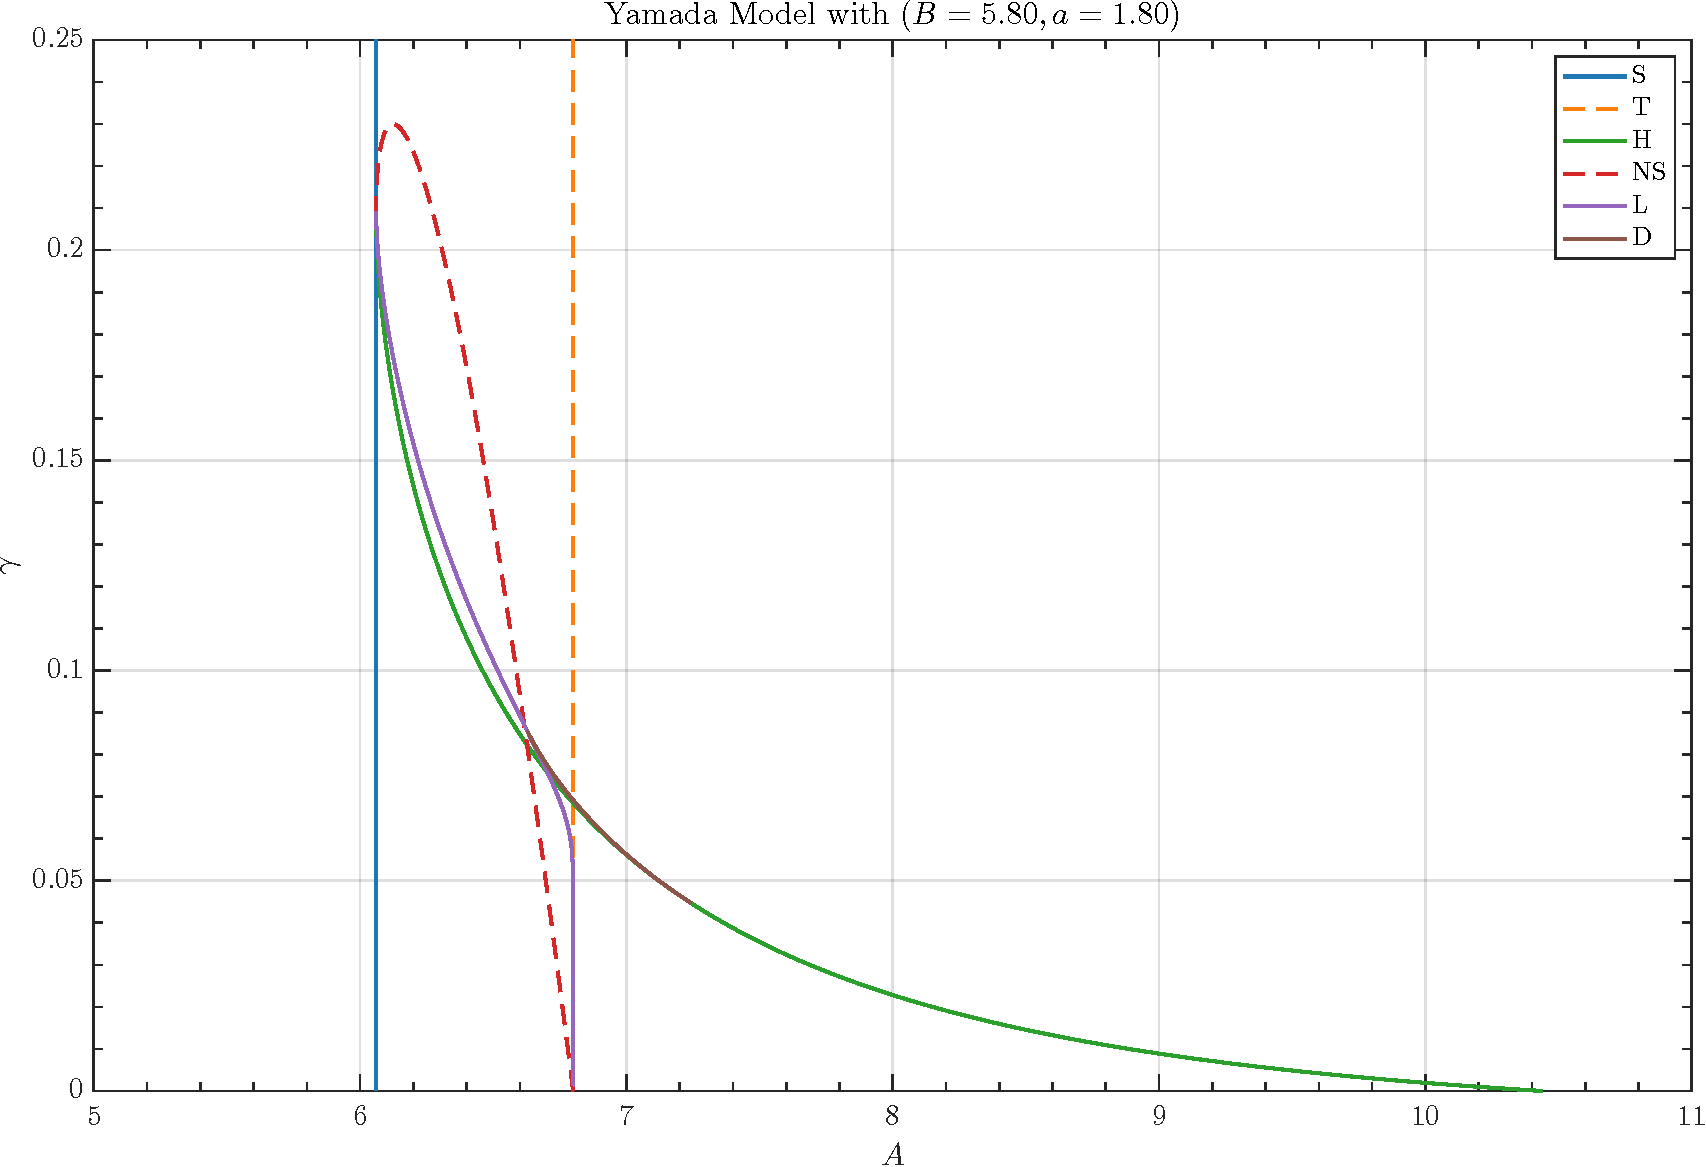
\includegraphics[width=\linewidth]{./images/bifurcations}
  \end{subfigure}
  ~
  \begin{subfigure}{0.48\linewidth}
    \caption{}
    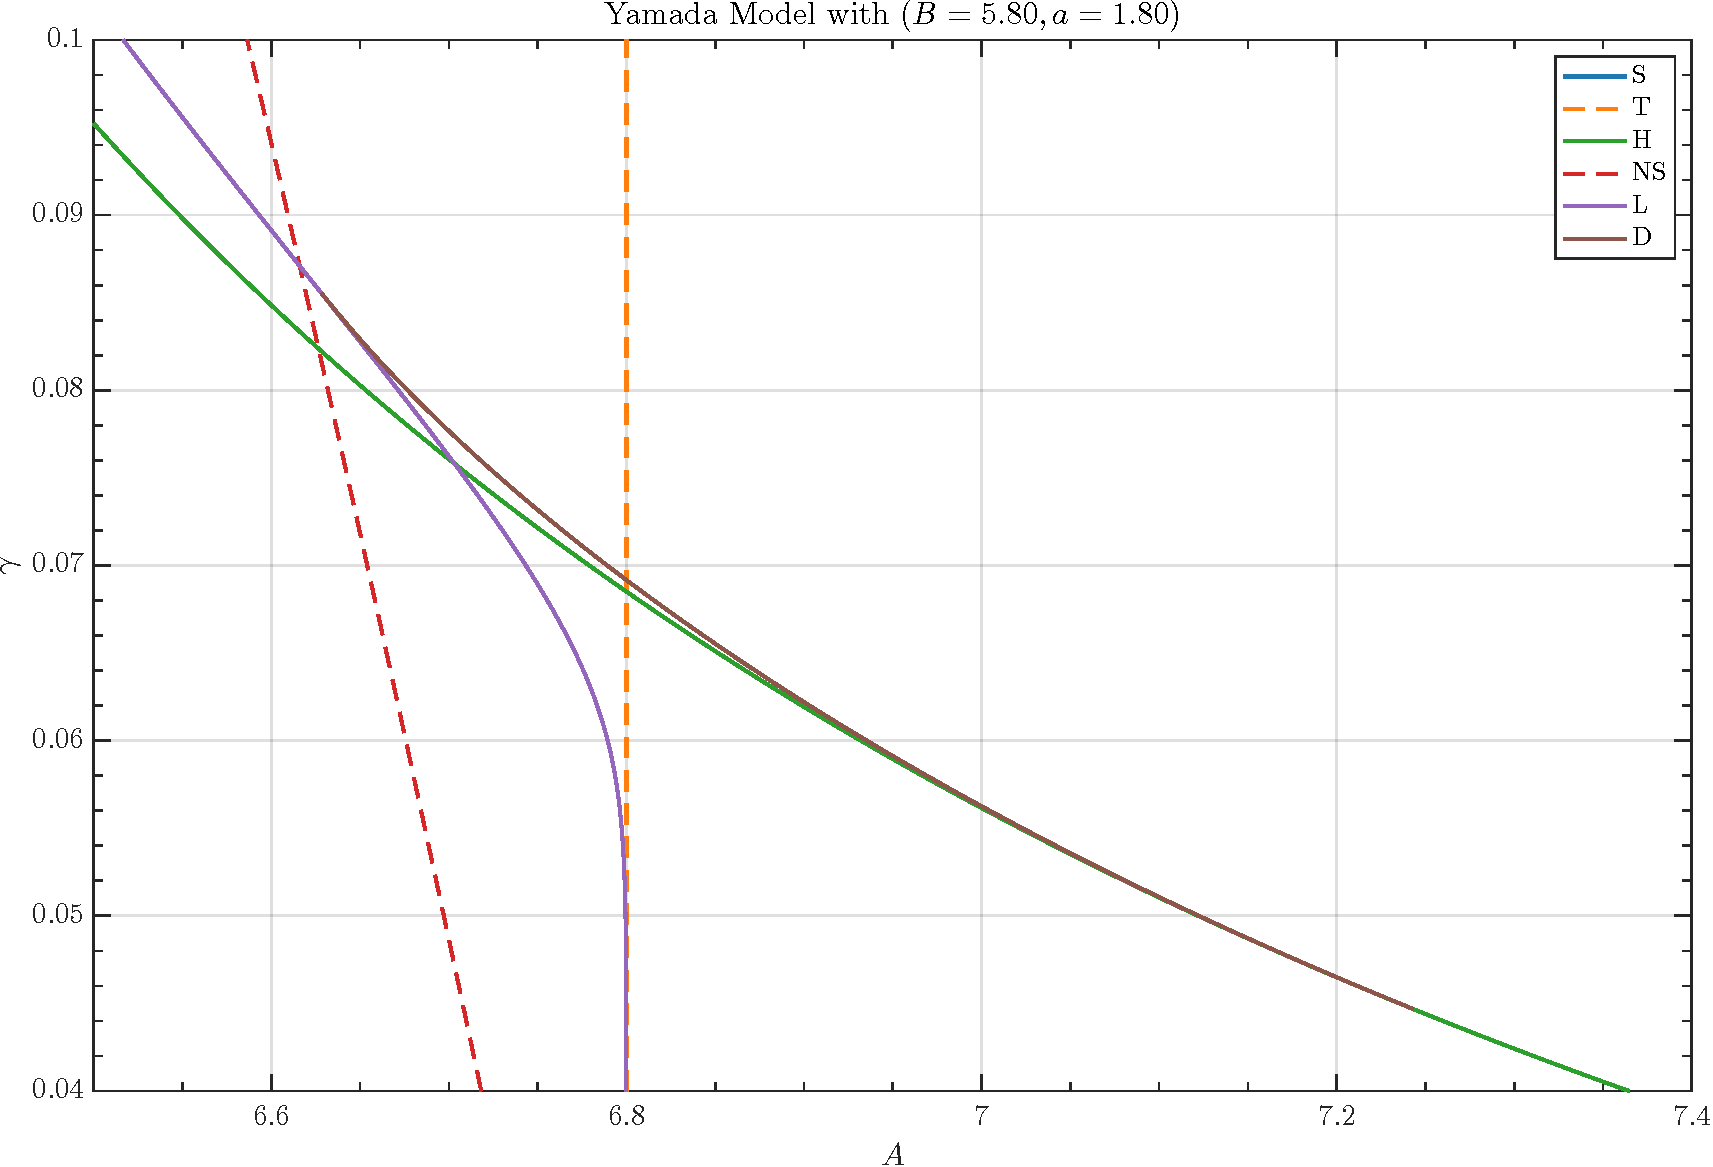
\includegraphics[width=\linewidth]{./images/bifurcations_zoomed}
  \end{subfigure}
  \caption{(a) Bifurcation diagram of the Yamada model. (b) Zoom-in of (a).}
  \label{fig:bifurcation_diagram}
\end{figure}

\section*{Phase-Resetting Segments}

We calculate the phase-resetting problem as four different segments.
\begin{itemize}
  \item $T$ is the period of the attracting periodic orbit,
  \item $\vec{x}_{i}$ is the state-space vector for segment $i$,
  \item $\vec{w}_{i}$ is the left-eigenvector of the Jacobian for segment $i$,
  \item $\theta_{\mathrm{old}}$ is the phase/point along the periodic orbit where the perturbation is applied,
  \item $\theta_{\mathrm{new}}$ is the phase/point long the periodic orbit where the perturbed segment as returned,
  \item $k$ is the periodicity of the perturbed segment,
  \item $A_{\mathrm{p}}$ is the perturbation amplitude
  \item $\vec{d}_{\mathrm{p}} = \left( \mathrm{cos}(\theta_{\mathrm{p}}) , 0 , \mathrm{sin}(\theta_{\mathrm{p}}) \right)$ is the perturbation directional vector, only applied in the $G-I$ plane.
\end{itemize}

\textbf{Segment 1} (\verb!func_seg1!)
\begin{subequations}
  \begin{gather}
    \vec{u}_{1} = \left( \vec{x}_{1}, \vec{w}_{1} \right) , \\
    \dot{\vec{x}}_{1} = T \theta_{\mathrm{new}} \vec{F} (\vec{x}_{1}) , \\
    \dot{\vec{w}}_{1} = -T \theta_{\mathrm{new}} D_{\vec{x}_{1}} \vec{w}_{1},
  \end{gather}
\end{subequations}

\textbf{Segment 2} (\verb!func_seg2!)
\begin{subequations}
  \begin{gather}
    \vec{u}_{2} = \left( \vec{x}_{2}, \vec{w}_{2} \right) , \\
    \dot{\vec{x}}_{2} = T \left( 1 - \theta_{\mathrm{new}} \right) \vec{F} (\vec{x}_{2}) , \\
    \dot{\vec{w}}_{2} = -T \left( 1 - \theta_{\mathrm{new}} \right) D_{\vec{x}_{2}} \vec{w}_{2},
  \end{gather}
\end{subequations}

\textbf{Segment 3} (\verb!func_seg3!)
\begin{subequations}
  \begin{gather}
    \vec{u}_{3} = \vec{x}_{3} ,\\
    \dot{\vec{x}}_{3} = T \left( 1 - \theta_{\mathrm{old}} \right) \vec{F} (\vec{x}_{3}) .
  \end{gather}
\end{subequations}

\textbf{Segment 4} (\verb!func_seg4!)
\begin{subequations}
  \begin{gather}
    \vec{u}_{4} = \vec{x}_{4} , \\
    \dot{\vec{x}}_{4} = k T \vec{F} (\vec{x}_{4}) .
  \end{gather}
\end{subequations}

\textbf{Boundary conditions}

The boundary conditions are separated into three files.

\verb!bcs_seg1_seg2!
\begin{subequations}
  \begin{gather}
    \vec{x}_{1}(0) - \vec{x}_{2}(1) = 0 , \\
    \vec{x}_{1}(1) - \vec{x}_{2}(0) = 0 , \\
    \hat{\vec{e}}_{1} \cdot \vec{F} (\vec{x}_{1}) = 0, \\
    \vec{w}_{1}(0) - \vec{w}_{2}(1) = 0 , \\
    \mu_{s} \vec{w}_{2}(0) - \vec{w}_{1}(1) = 0 , \\
    \left\| \vec{w}_{2}(0) \right\| - 1 = 0 .
  \end{gather}
\end{subequations}

\verb!bcs_seg3!
\begin{equation}
  \vec{x}_{3}(1) - \vec{x}_{1}(0) = 0 .
\end{equation}

\verb!bcs_seg4!
\begin{subequations}
  \begin{gather}
    \vec{x}_{4}(0) - \vec{x}_{3}(0) - A_{\mathrm{p}} \vec{d}_{\mathrm{p}} = 0 , \\
      \left( \vec{x}_{4}(0) - \vec{x}_{2}(0) \right) \cdot \vec{w}_{2}(0) = 0 , \\
      \left\| \vec{x}_{4}(1) - \vec{x}_{2}(0) \right\|^{2} - \eta = 0.
  \end{gather}
\end{subequations}
We write the final boundary condition as the norm-squared to avoid a singularity in the Jacobian :)

\end{document}
%==============================================================================%
%                                 END DOCUMENT                                 %
%==============================================================================%